\chapter{Stabilizing Value Function Learning with Model-Generated Data}
\label{chap:mad}

\begin{quote}
    This chapter is based on \longfullcite{voelcker2025mad}.
\end{quote}


\newcommand{\blue}[1]{{\color{uoftoceanblue} #1}}
\newcommand{\red}[1]{{\color{uoftred} #1}}

\section{Introduction}

% Introducing the setting -- off policy rl - and the problem
Instead of solely relying on data gathered by a target policy, \emph{off-policy} reinforcement learning (RL) aims to leverage experience gathered by past policies \parencite{sutton2018introduction} to fit a value function for the target policy. 
Ideally, training over many iterations should help extract important information from past data.
However, recent work has shown that simply increasing the number of gradient update steps, the \emph{replay ratio} or \emph{update-to-data (UTD) ratio}, can lead to highly unstable learning~\parencite{nikishin2022primacy,doro2023barrier,hussing2024dissecting,nauman2024bigger}.

% Introducing prior attempts to fix the problem
% To address this issue, 
Prior work has stabilized the learning by using double Q minimization to reduce overestimation \parencite{fujimoto2018addressing}, training ensemble methods to improve value estimation \parencite{chen2020randomized,hiraoka2022dropout}, introducing architectural regularization \parencite{hussing2024dissecting,nauman2024bigger}, or resetting networks periodically throughout the learning process \parencite{doro2023barrier,schwarzer2023bigger,nauman2024bigger}.
However, while useful, pessimistic underestimation and architectural regularization are insufficient by themselves  to combat the problem \parencite{hussing2024dissecting}, and so most methods resort to either network resets or ensembles.
Critic ensembles can be expensive to train, and resetting has several important limitations: in real systems, re-executing a random policy can be expensive or unsafe, the resetting interval needs to be carefully tuned \parencite{hussing2024dissecting}, and when storing a full reset buffer is infeasible, resetting loses important information.

% Our main insight
We narrow in on a key issue contributing to unstable training: \emph{wrong value function estimation on unobserved on-policy actions} \parencite{thrun1993issues,tsitsiklis1996analysis}.
Off-policy RL uses the values of states sampled under old policies with actions from the target policy to update the value function.
However, these state-action pairs themselves are not in the replay buffer and hence their value estimate is not directly improved by training.
Consequently, a learned function which achieves low error on seen data is not guaranteed to generalize well to actions that \emph{differ} from past actions.
This problem is related to overfitting \parencite{li2023efficient} and contributes to overestimation \parencite{thrun1993issues,hasselt2010double,fujimoto2018addressing}.
However, overfitting assumes that train and test set are drawn from the same distribution, while we focus on the distribution shift between data collection and target policy.
Previous work has investigated the difficulty of off-policy learning due to this shift~\parencite{maei2009convergent,sutton2016emphatic,hasselt2010double,fujimoto2018addressing}, yet there are no tractable mitigation strategies that work well in the high UTD regime with deep RL.

% what we did to obtain the insight and the solution
To corroborate our hypothesis that generalization to unobserved actions is a major obstacle for training at high UTDs, we examine the behavior of value functions on on-policy transitions. 
Our experiments reveal that value functions generalize significantly worse to unobserved on-policy action transitions than to validation data from the same distribution as the training set.
Building on this, we propose to improve on-policy value estimation by using \emph{model-generated on-policy data}.

Previous investigations into model-based deep RL have focused on learning values fully in model roll-outs \parencite{buckman2018sample,janner2019mbpo,hafner2020dream,ghugare2023simplifying} and the associated challenges~\parencite{zhao2023simplified,hansen2024tdmpc}.
In contrast, we show that mixing a small amount of model-generated on-policy data with real off-policy replay data is sufficient to achieve stable learning in the high UTD regime.
Our method, Model-Augmented Data for TD learning (MAD-TD), mitigates the generalization issues of the value function in the hardest tasks of the DeepMind control (DMC) benchmark~\parencite{tunyasuvunakool2020dmcontrol} and achieves strong and stable high UTD learning without resetting or redundant ensemble learning. 

The main contributions of this work are twofold:
First, we empirically show the existence of misgeneralization from off-policy value estimation to on-policy predictions. We connect this issue to the challenge of stable learning with high update ratios and highlight how increasing the update ratio increases Q function overestimation.
Second, we provide a new method called MAD-TD that improves the value function accuracy on unobserved on-policy actions with model-generated data and stabilizes training at high update ratios. This method proves to have equivalent performance to or outperform previous strong baselines.

\section{Off-policy value function learning}

Many algorithms attempt to simplify the direct policy optimization problem by first learning a policy value function $Q^\pi$, which is defined via a recursive equation% \footnote{Note that due to the assumption of a deterministic environment, the expectation simplifies to a simple function evaluation.} 
\begin{equation*}
Q^\pi(x,a) = r(x,a) + \gamma \mathbb{E}_{x' \sim \mathcal{P}(\cdot|x,a), a' \sim \pi(\cdot|x')}\left[Q^\pi(x',a')\right]\enspace.    
\end{equation*}
The policy can then be incrementally improved by picking 
% \begin{align}
% \pi_{k+1}(x) \in \argmax_{\mathcal{A}} Q^{\pi_k}(x,a)\label{eq:mad:pi_update}
% \end{align}
$\pi_{k+1}(x) \in \argmax_{a \in \mathcal{A}} Q^{\pi_k}(x,a)\label{eq:mad:pi_update}$
at every time step $k$.
In practice, $Q^\pi$ and $\pi$ are often parameterized as neural networks and learned from data. 
To increase the sample efficiency of the algorithm, it is common to store \textit{all} collected interaction data independent of the collection policy in a replay buffer $\mathcal{D} = \{(x_t, a_t, r_t, x_{t+1})_{t=0}^{T}\}$.
As the Q-value only depends on the policy via the policy evaluation at the next state, it is possible to estimate Q-values from past interaction data by minimizing the fitted Q-learning objective 
\begin{align}
\mathcal{L}\left(\hat{Q}\middle|\blue{\mathcal{D}}, \pi\right) = \frac{1}{|\mathcal{D}|} \sum_{t=0}^T \left| \hat{Q}(\blue{x_t,a_t}) - \left[\blue{r_t} + \gamma \hat{Q}\left(\blue{x_{t+1}}, \red{a'}\right)\right]_\mathrm{sg} \right|^2\quad \mathrm{with }~\red{a'}\sim \pi(\cdot|\blue{x_{t+1}}) \enspace. \label{eq:mad:off_policy_q_update}
\end{align}
Here $[\cdot]_\mathrm{sg}$ denotes the stop gradient operation introduced to avoid the double sampling bias and all data contained in the replay buffer is colored \blue{blue}. 
% In practice $\hat{Q}$ is parameterized with neural networks, and the objective is minimized over randomly sampled mini-batches with a modern gradient learning algorithm such as Adam.
However, the Q value at the next state $\blue{x_{t+1}}$ is evaluated with an action $\red{a'}$ that is \emph{not} guaranteed to be in the replay memory, as the target policy can be different from the policy used to gather the sample.
This means that we require the Q value to generalize to potentially unseen actions.
We provide a visualization of this issue in~\autoref{fig:mad:mad:coverage}.

\section{Investigating the root cause of unstable Q learning}

\begin{figure}[t]
\begin{minipage}{0.6\textwidth}
    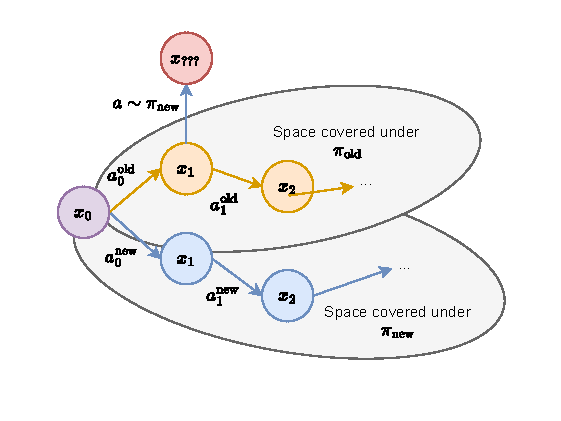
\includegraphics[width=\textwidth]{illustrations/mad-td/rl_sequences.drawio.pdf}
\end{minipage}
~
\begin{minipage}{0.39\textwidth}
    \caption{A visualization of the core issue we investigate. Even if a replay buffer contains good coverage for two policies ($\pi_\mathrm{old}$ and $\pi_\mathrm{new}$) starting from $\rho=x_0$, this does not guarantee that it contains a transition for executing an action under the new policy on a state visited under the old. However, this state-action pair's value estimate is used to update the value of state $x_0$ via \autoref{eq:mad:off_policy_q_update}, without being grounded in an observed transition.}
    \label{fig:mad:mad:coverage}
\end{minipage}
\end{figure}
    

Minimizing \autoref{eq:mad:off_policy_q_update} finds the policy Q function over a replay buffer with sufficient coverage of all states and actions that this policy visits.
However, in most continuous control RL algorithms~\parencite{ddpg,haarnoja2018sac, fujimoto2018addressing}, this update is interleaved with policy update steps .
The data in $\mathcal{D}$ then necessarily becomes \emph{off-policy} as training progresses. 

This means that the number of actor and critic optimization steps needs to be balanced with gathering new data.
Obtaining new on-policy data is vital to continually improve policy performance \parencite{ostrovski2021difficulty}, but performing more update steps before gathering new data ensures that the existing data has been used effectively to improve the policy.
The \emph{replay ratio} \parencite{fedus2020revisiting} or \emph{update-to-data (UTD) ratio} \parencite{nikishin2022primacy}, which governs the number of gradient steps per environment step, is therefore a vital hyperparameter.

Naively training with high UTD ratios can lead to collapse in off-policy deep RL \parencite{nikishin2022primacy}.
We conjecture that one of the major causes of the instability of high UTD off-policy learning are wrong Q values on \emph{unobserved actions}.
This is a well-known problem for off-policy TD learning \parencite{baird1995residual,tsitsiklis1996analysis,sutton2016emphatic,ghosh2020representations}.
To differentiate the problem from \emph{overfitting} to the training distribution, we use the term \emph{misgeneralization} to highlight the importance of the distribution shift in causing the issue.
Our experiments in \autoref{sec:mad:off-policy-eval-exp} show that generalization to on-policy actions is more difficult than generalization to a validation dataset that follows the training distribution, and that higher UTDs exacerbate the issue.

\subsection{Action distribution shift can cause off-policy Q value divergence}
\label{sec:mad:theory}
To highlight the role that on-policy actions play in stabilizing Q value learning, we show an analysis the stability of Q learning with linear features.
The core ideas follow \textcite{sutton2016emphatic} and are also explored by \textcite{tsitsiklis1996analysis,sutton1988learning}.
We assume that the Q function is parameterized with fixed features and weights as $Q(x,a) = \phi(x,a)^\top \theta$.
Let $X$ and $A$ be the sizes of the state and action space respectively. Let $P \in \mathbb{R}^{X\cdot A \times X}$ be the matrix of transition probabilities from state-action pairs to states.
A policy can then be expressed as a mapping $\Pi \in \mathbb{R}^{X\times X\cdot A}$ from states to the likelihood of taking each action.
$R \in \mathbb{R}^{X\cdot A}$ is the vector of rewards.
$D^{\pi} \in \mathbb{R}^{X\cdot A \times X\cdot A}$ is a matrix where the main diagonal contains the discounted state-action occupancies of $P^\pi$ starting from $\rho$.
If we assume access to a mixed replay buffer $\mathcal{D} = \bigcup \{D^{\pi_1}, \dots, D^{\pi_n}\}$ gathered with different policies, the Q learning loss for a target policy $\Pi$ can be written as
\begin{align}
    L(\theta) = & \sum_{i=1}^n \left[D^{\pi_i}\left(\Phi^\top \theta - [R + \gamma P\Pi \Phi^\top \theta]_\mathrm{sg}\right))^2\right] \enspace.
\end{align}
The stability of learning with this loss can be analyzed using the gradient flow
    \begin{align}
    %&= 2 \Phi \sum_{\pi_b} d^{\pi_b} \left(\left(I - \gamma P \Pi \right)\Phi^\top \theta - R\right)\\
    \dot{\theta} &= - 2 \Phi \sum_{i=1}^n D^{\pi_i} \left(I - \gamma P\Pi \right)\Phi^\top \theta + 2 \Phi \sum_{i=1}^n D^{\pi_i} R \enspace.
\end{align}
This gradient flow is guaranteed to to be stable around a fixed point $\theta^*$ if the key matrix $\sum_{i=1}^n D^{\pi_i} \left(I - \gamma P \Pi \right)$ is positive definite \parencite{sutton1988learning}. 
Details and a proof of the following statement are provided in \autoref{app:math}.
We can decompose the key matrix and see that the positive definiteness depends on the difference in policy between the replay buffer and the target policy
\begin{align}
    \sum_{i=1}^n D^{\pi_i} \left(I - \gamma P\Pi \right) = \blue{\underbrace{\sum_{i=1}^n D^{\pi_i} \left(I - \gamma P\Pi_i \right)}_{\text{positive definite}}} + \gamma \red{\underbrace{\sum_{i=1} D^{\pi_i}P (\Pi_i - \Pi)}_{\text{no guarantees}}} \enspace .
\end{align}
%\ee{Can we make it obvious that the ??? above is intentional rather than a latex error? What about replacing with "no guarantees"?}
In general, we can provide no guarantees for the \red{second term} outside of the on-policy case ($\Pi_i = \Pi)$ where it becomes $0$.
The stability depends on the difference between the target policy and the data-collection policies.
If the target policy takes actions which are not well covered under the training policies, the remainder can be non positive definite.
This also matches the intuition that learning fails if we simply do not have sufficient evidence for the Q function of unobserved actions.

When using features, the eigenvalue conditions on the key matrix are only sufficient, not necessary, as the features can allow for sufficient generalization between observed and unobserved state-action pairs.
In deep RL, the features $\phi$ are updated alongside with the weights, making it hard to provide definitive mathematical statements on stability.
With good function approximation, we could hope that the learned value function generalizes correctly to unseen actions.
In the next section we investigate this for a non-trivial task from the DMC suite and highlight that, while the value function does not diverge irrecoverably, good generalization is not guaranteed either. % \mh{need to bring this back to intuition otherwise people will ask of us to measure eigenvalues}

\subsection{Empirical Q value estimation with off-policy data}
\label{sec:mad:off-policy-eval-exp}

% 
% \begin{enumerate}
%     \item Get two different policies on difficult task
%     \item Learn Q values on policy
%     \item Show that these don't generalize between the two policies
%     \item We can even estimate ground truth MC style
% \end{enumerate}
% 
% \mh{Highlight that this is not overestimation. On training data we are accurate. Differentiate between overfitting, overestimation, and misgeneralization.}
\begin{figure}[t]
\begin{minipage}{0.25\textwidth}
    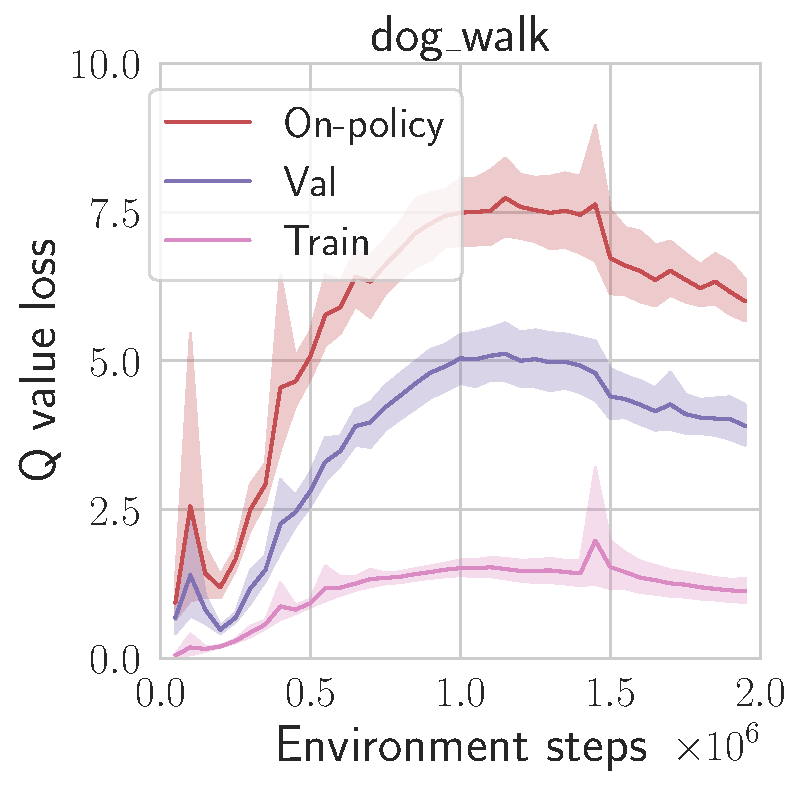
\includegraphics[width=\textwidth]{figures/mad-td/critic_loss_dog_walk.pdf}
\end{minipage}
~
\begin{minipage}{0.745\textwidth}
    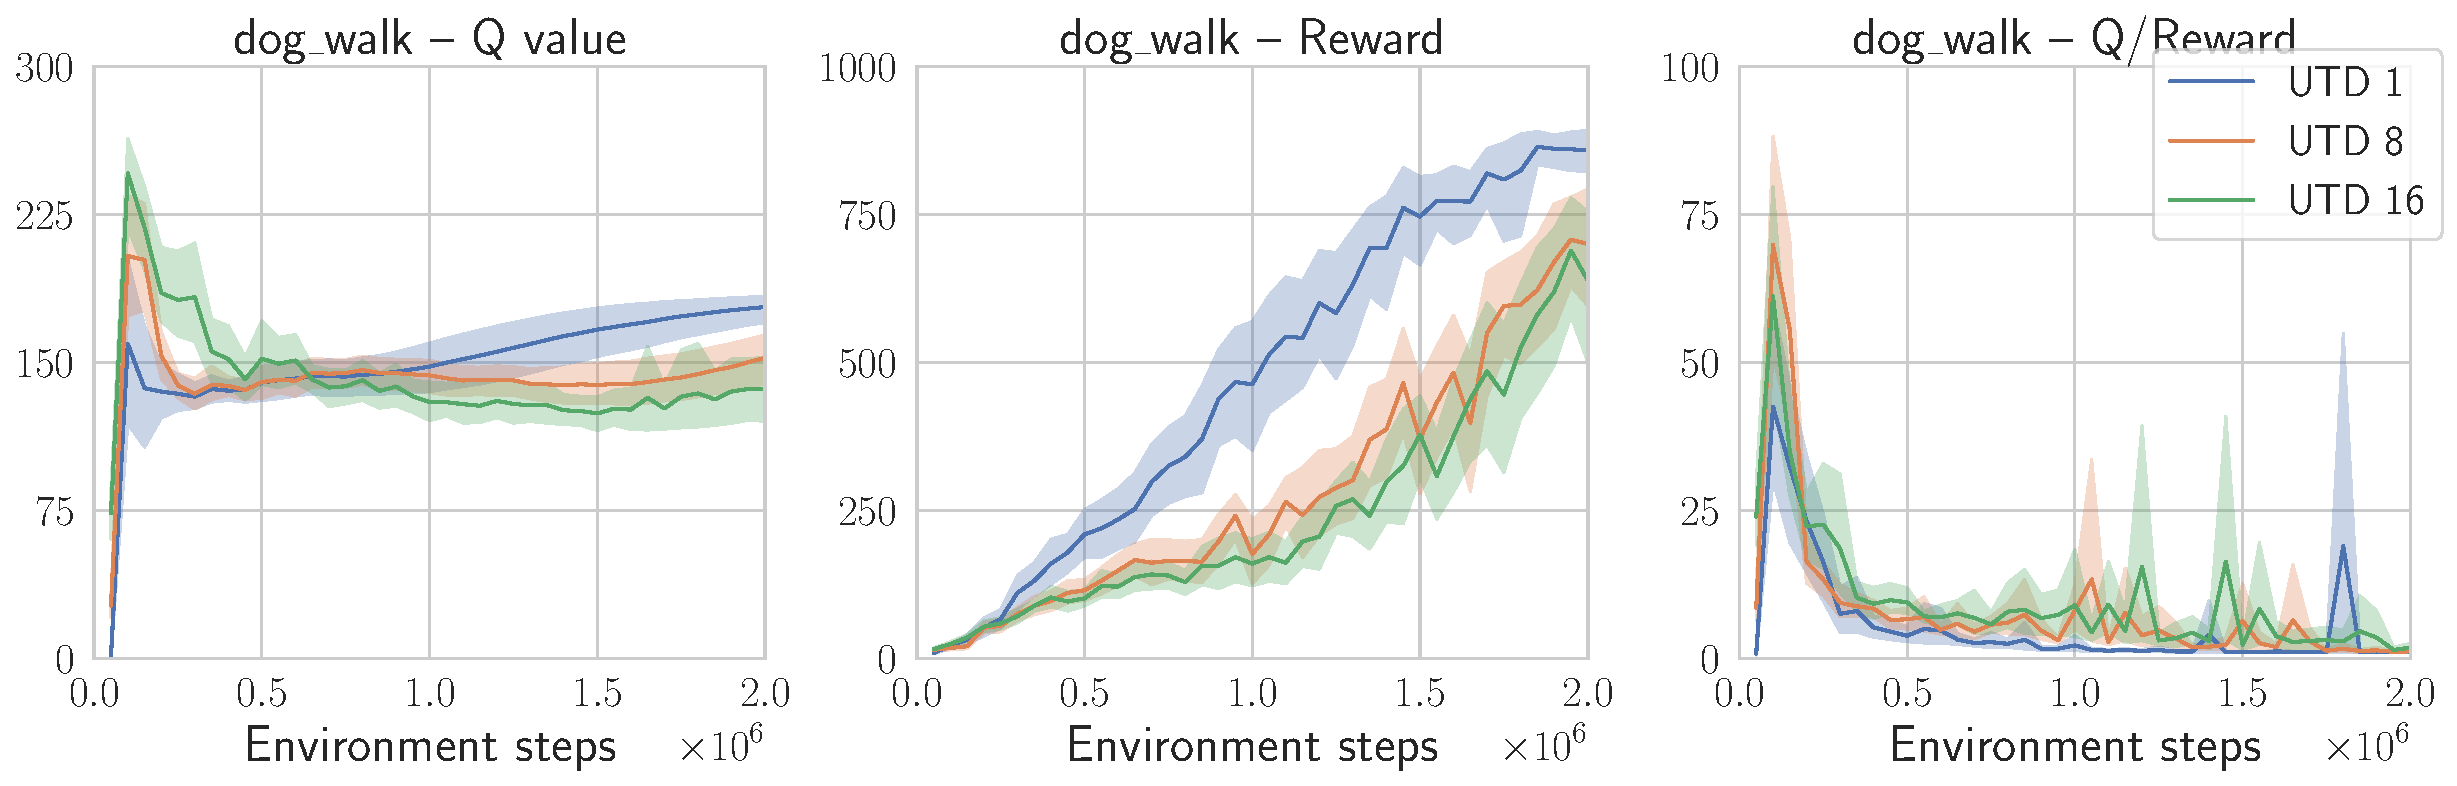
\includegraphics[width=\textwidth]{figures/mad-td/q_overestimation.pdf}
\end{minipage}
\caption{Left: the \sbcpink{train}, \sbcpurple{validation}, and \sbcred{on-policy} validation error of the Q function at UTD 1. Right: the Q values and return curves of TD3 agents across different UTD \sbcblue{1}, \sbcorange{8}, and \sbcgreen{16}.}
\label{fig:mad:q_eval}
\end{figure}

In environments with large state-action space, ensuring coverage is difficult.
To investigate whether learning is stable nonetheless, we train a model-free TD3 agent on the \emph{dog walk} environment \parencite{tunyasuvunakool2020}.
The architecture is presented in \autoref{sec:mad:method}, and is regularized to prevent catastrophic divergence \parencite{hussing2024dissecting,nauman2024overestimation} and uses clipped double Q learning \parencite{fujimoto2018addressing}.
This means it uses the most common techniques which are designed to prevent misgeneralization and overestimation.
% We choose this task as the model-free agent obtains good performance across UTDs.

While training a TD3 agent \parencite{fujimoto2018addressing}, we save transitions in a validation buffer with a 5\% probability.
At regular intervals we compute the critic loss on this validation set.
In addition, we reset our simulator to each validation state and sample an action from the target policy.
We then simulate the ground truth on-policy transition and compute the loss over these.
This allows us to test how well our value function generalizes to target policy state-action pairs (as depicted in~\autoref{fig:mad:mad:coverage}).
% This procedure is not applicable in regular RL training which assumes that the simulator is not under the control of the agent, but it provides insights into the behavior of Q learning.
% With these new transitions, we can compare the validation loss, which is computed on a distribution similar to the training dataset, and the generalization loss to on-policy actions.

The results are presented in \autoref{fig:mad:q_eval} and show a gap both between the train and validation sets, as well as the validation and the on-policy sets.
While we use the on-policy state-actions to update the Q value, these estimates are not actually consistent with the environment.
Furthermore, the Q value overestimation grows with increasing UTDs.
This phenomenon was previously discussed in the context of over-training on limited data \parencite{hussing2024dissecting} .

The experiments show that the problem outlined in \autoref{sec:mad:theory} is not merely a mathematical curiosity, but that Q value generalization to out-of-replay-distribution actions is difficult in practice, and becomes more difficult with increasing update ratios.
Even though full divergence is not observed as new data is continually added to the replay buffer, it takes a long time for the effects of severe early overestimation to dissipate.

\subsection{Previous attempts to combat misgeneralization and overestimation}
\label{sec:mad:prior}
% To mitigate the effects of value function misgeneralization, several recent works have developed strategies to deal with this issue.
Prior strategies that deal with misgeneralization can be grouped into three major directions: architectural regularization to prevent divergence of the value function, pessimism or ensemble learning to combat overestimation, and networks resets to restart learning.
While all of these interventions help to some degree, they each either do not solve the problem in full or cause additional issues.

\textbf{Architectural regularization}~~~Architecture changes \parencite{hussing2024dissecting,nauman2024overestimation,nauman2024bigger,lyle2024disentangling} and auxiliary feature learning losses \parencite{schwarzer2021dataefficient,zhao2023simplified,ni2024bridging,voelcker2024when} are largely reliable interventions, and have shown to provide improvements without much drawbacks in prior work.
However, as \textcite{hussing2024dissecting} and our experiment presented in \autoref{sec:mad:off-policy-eval-exp} highlight, by themselves they can mitigate catastrophic overestimation and divergence, but do not guarantee proper generalization. %{\color{red} EE: Awkward phrasing on the end of this sentence} \cv{Better?}
%In this work, we use the TD-MPC2 architecture which interleaves layer normalization with a softmax normalized encoding layer.

\textbf{Pessimism and ensembles}~~~To combat overestimation directly, the most prominent approach in continuous action spaces is Clipped Double Q Learning \parencite{fujimoto2018addressing}. 
Here, a Q value estimate is obtained from two independent estimates $\hat{Q}_1$ and $\hat{Q}_2$.
If the error of the two critic estimators is assumed to be independent noise on the true critic estimate 
%$\hat{Q}_{1/2} = Q + \epsilon_{1/2}$, 
then using the minimum over both estimates is guaranteed to underestimate the true critic value in expectation.
However, in complex settings this assumption on the the error of the critic estimates may not hold. 
%Furthermore, using two critics can be overly pessimistic \parencite{}.

Ensembles \parencite{lan2020maxmin,chen2020randomized,hiraoka2022dropout,farebrother2023protovalue} or online tuning of the rate of pessimism \parencite{moskovitz2021tactical} have been proposed to obtain tighter lower bounds on the Q value.
However, these strategies can be expensive as redundant models or hyperparameter tuning are needed.
As a simpler strategy, recent works have also employed clipping to obtain an upper bound of the Q function to prevent divergence \parencite{fujimoto2024sale}.

\textbf{Resetting}~~~Finally, network resets been shown to mitigate training problems \parencite{nikishin2022primacy,doro2023barrier,schwarzer2023bigger,nauman2024bigger} in high UTD regimes.
However, in cases where the agent fails to explore any useful parts of the state space within the reset interval, restarting the learning process will not improve performance \parencite{hussing2024dissecting}.
This makes tuning the resetting interval both important and potentially difficult and no tuning recipes have been presented.
Resetting is also a potentially hazardous strategy in real-world applications, where re-executing a random policy might be costly or infeasible due to safety constraints.
Finally, it heavily relies on the assumption that all past interaction data can be kept in the replay buffer.

% While all of these approaches can help to reduce overestimation and stabilize learning, the root cause ofcan fail to generalize, even if the magnitude of the Q value is controlled~\mh{missing citation or pointer}.
All of these strategies are somewhat able to alleviate the problem of out-of-distribution value estimation, yet none of them directly address the issue at the root.
In the next chapter, we present an alternate approach that aims to directly regularize the action value estimates under the target policy.
% \mh{Combine this paragraph with the last one of pessimism}

\section{Mitigation via model-generated synthetic data}

As value functions misgeneralize due to lack of sufficient on-policy data, we propose to obtain synthetic data from a learned model instead.
However, model-based RL can also cause problems such as compounding world model errors and optimistic exploitation of errors in the learned model. 
By using both real and model-generated data, we can trade-off these issues: on-policy data improves the value function and limits the impact of off-policy distribution shifts, while using only a limited number of model-generated samples prevents model errors from deteriorating the value estimates. 

Our approach builds on the TD3 algorithm \parencite{fujimoto2018addressing} and uses an update ratio of 8 by default. 
Our critic is updated with both model-based and real data following the DYNA framework \parencite{dyna}.
More precisely, we replace a small fraction $\alpha$ of samples $\{x,a,r,x'\}$ in each batch with samples from a learned model $\hat{p}$ starting from the same state $\{x, \pi(x), \hat{r} ,\hat{x}'\}$ with $\hat{r}, \hat{x}' \sim \hat{p}(\cdot|x, \pi(x))$. In our experiments, $\alpha$ is set to merely $5\%$.
We term this approach Model-Augmented Data for TD learning ~(MAD-TD).% \mh{i changed this to mad td, but not sure about full name} 

\textbf{Model vs Q function generalization}~~~We expect that a learned models will yield better generalization than the Q function for two reasons.
First, the policy is updated each step to find an action that maximizes the value function.
This means we are effectively conducting an adversarial search for overestimated values.
The model's reward and state estimation error on the other hand are independent of this process.
We test the adversarial robustness of our model-augmented value functions in \autoref{sec:mad:adv_robustness}.
Second, our experiment shows that value functions primarily diverge at the beginning of training.
In these cases, coverage is low and on-policy state-action pairs are often not available.
Obtaining a slightly wrong, yet converging value estimate can then be more useful than a diverging one. 
Even as more data is gathered, new policies might not revisit old states with a high likelihood.
Therefore even as training continues we expect the model data to provide some benefit.

\subsection{Design choices and training setup}
\label{sec:mad:method}

Our model is based on the successful TD-MPC2 model \parencite{hansen2024tdmpc} combined with the deterministic actor-critic algorithm TD3 \parencite{fujimoto2018addressing}.
We aim to reduce the complexity of TD-MPC2 to the minimal necessary components to achieve strong learning in the DM Control suite, and thus forgo added exploration noise, SAC, ensembled critics, and longer model rollout for training or policy search. We outline several design choices here and refer to \autoref{app:setup} for more detail.

\textbf{Encoder:}~~~~Like TD-MPC2, we parameterize the state with a learned encoder $\phi: \mathcal{X} \rightarrow \mathcal{Z}$ with a SimNorm nonlinearity \parencite{lavoie2023simplicial}. 
% Formally, this function maps into the space of n k-dimensional simplices. 
This transformation groups a latent vector into groups of $k$ entries and applies a softmax transformation over each group.
This bounds the norm of the features, which has been shown aid with stable training \parencite{hussing2024dissecting,nauman2024overestimation}.

\textbf{Critic representation and loss:}~~~We use the HL-Gauss transformation to represent the Q function \parencite{farebrother2024stop}. The critic loss is the cross-entropy between the estimated Q function's categorical representation and the bootstrapped TD estimate.
To stabilize learning, we initialize the critic network towards predicting $0$ for all states.
We find that this stabilizes the initial update steps in which almost no data is available.

\textbf{Model loss:}~~~The world model predicts the next state latent representation and the observed reward from a given encoded state $\phi(x)$ and action $a$. The loss has three terms: the cross-entropy loss over the SimNorm representation of the encoded next state, the MSE between the reward predictions, and the cross-entropy between the next state critic estimate and the predicted state's critic estimate.
This final term replaces the MuZero loss in TD-MPC2 with a simplified variant based on the IterVAML loss \parencite{itervaml}.
We provide the exact mathematical equations for the loss in \autoref{app:implementation}.
%~\mh{too many inline equations imo} \cv{will change if space is available} \mh{maybe we can remove some of them? MSE of rewards and stuff probably does not have to written out, maybe just the complex ones} \cv{Last time I did that I got bonked by anal reviewers twice :D}

% \paragraph{Critic gradient} Previous work \cv{citation needed} claims that propagating the critic gradients to the encoder network leads to unstable training, we do not observe this issue and we include the critic loss in the first update step in the model update.
% We conjecture that this is due to the fact that our encoder is learned at a slower pace than the critic at high UTDs, and that our critic targets are significantly less wrong at the beginning of training, greatly stabilizing the updates.

\textbf{Training:}~~~We train the architecture by interleaving one environment step with one round of updates with a varying number of gradient steps governed by the UTD parameter.
For each update step, a new mini-batch is sampled independently from a replay buffer of previously collected experience.
We found that varying the number of update steps only for the critic and actor while keeping the update ratio for the model and encoder updates at $1$ leads to significantly more stable learning.

\textbf{Run-time policy improvement with MPC:}~~~Following the approach outlined by  \textcite{hansen2022temporal}, the learned model can also be used at planning time to obtain a better policy.
Using the model for MPC at planning time exploits the same benefit of models as the critic learning improvement: we obtain a model-corrected estimate of the value function and choose our policy accordingly.
As we only train our model for one step, we also conduct the MPC rollout for one step into the future.
% Note that in our current setup, we do not use the model uncertainty or an optimistic bonus to the value function, although following recent literature \parencite{bjorck2022is}, we use a mean over the double Q functions instead of the minimum within the MPC estimate.
%~\mh{do we actually still use the mean?} \cv{yes, I double checked, but only within MPC}.

%In keeping with our goal to present a minimalist approach, we only roll out our learned model for a single step into the future. We find that this is sufficient to not only obtain strong performance, but to obtain performance that is on par or in some cases even exceeds previously proposed resetting based methods in almost all environments.~\mh{dont think that is true for all exps, maybe delete this whole paragraph}

\section{Experimental evaluation}

\begin{figure}[t]
    \centering
    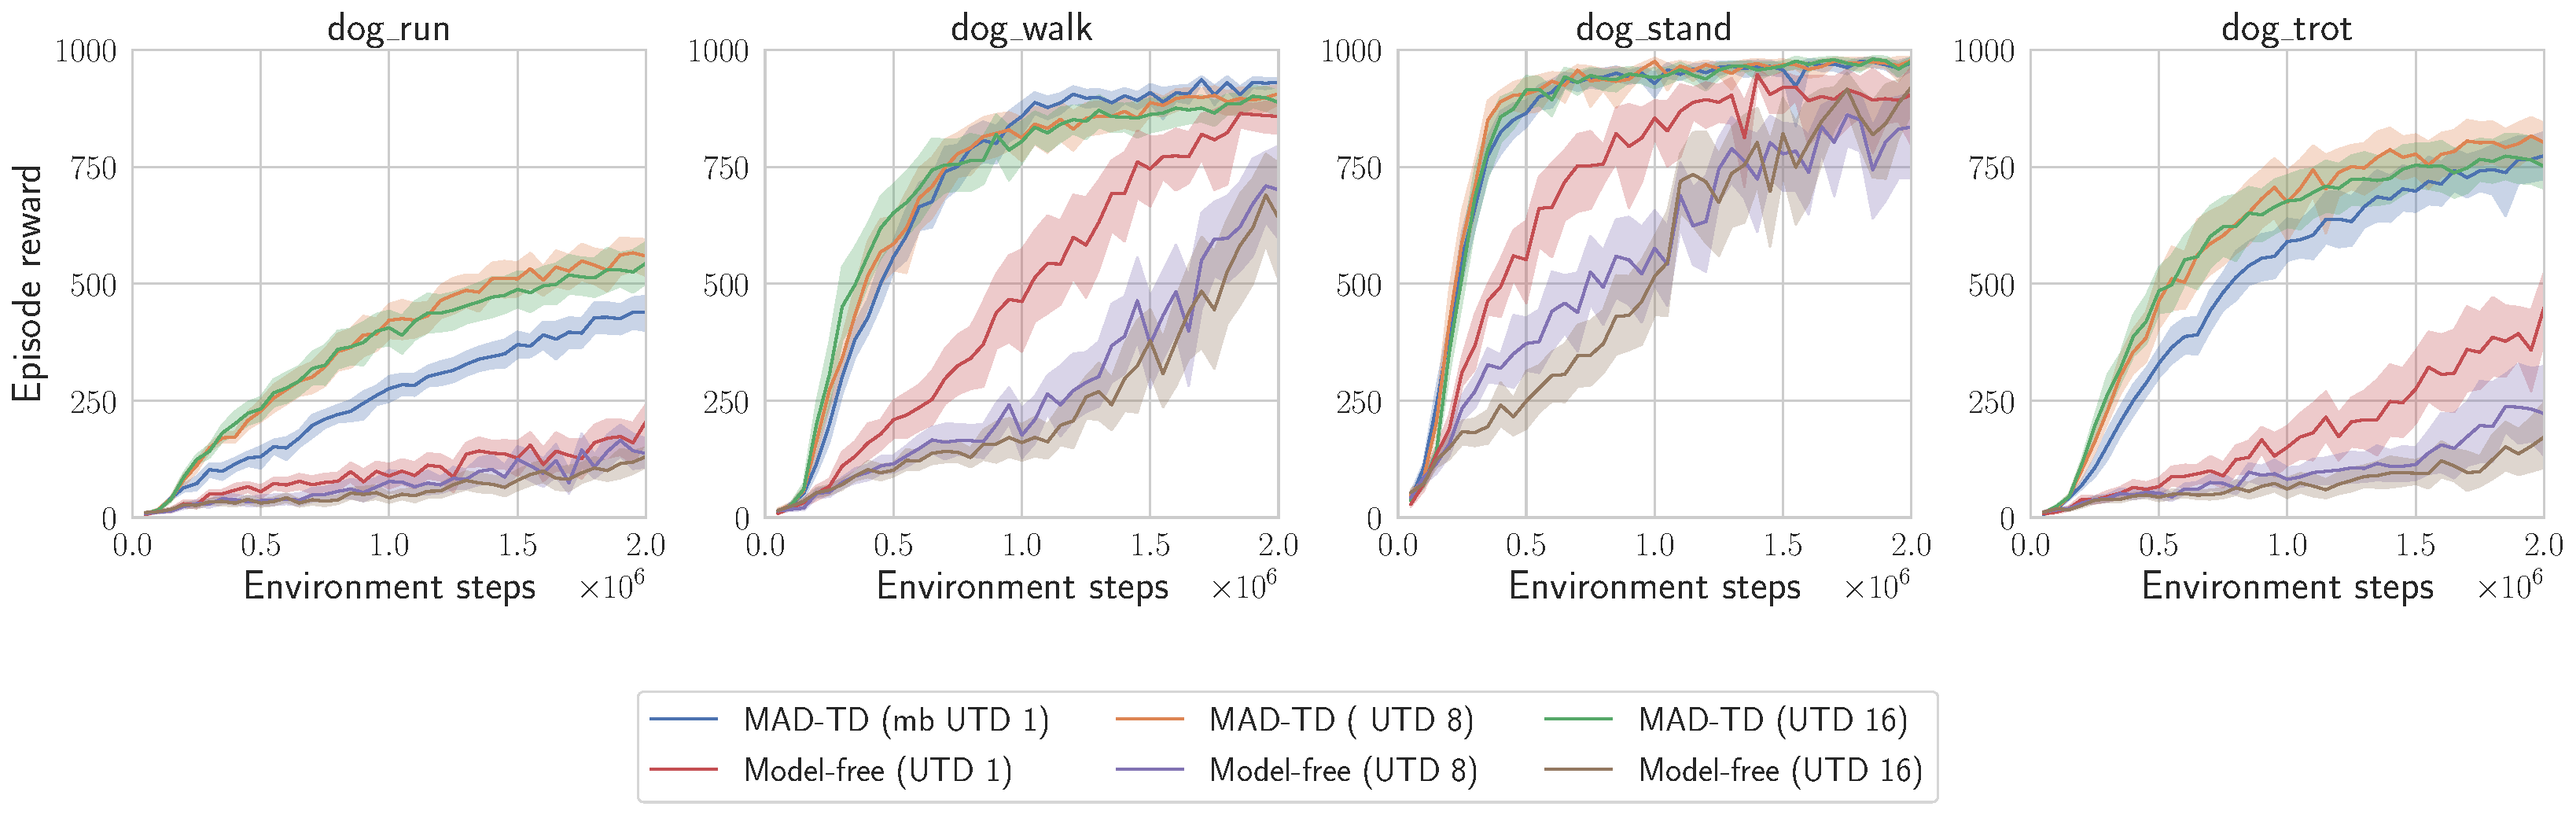
\includegraphics[width=1.0\linewidth]{figures/mad-td/dog_utd_comp.pdf}
    \caption{Return curves for the dog tasks with differing UTD values. Across all tested environments, the return increases or remains stable with increasing UTD when training with MAD-TD. Without model data, the performance decreases when increasing the UTD. MPC is turned off in these runs to cleanly evaluate the impact of model data on critic learning.}
    \label{fig:mad:main_dog}
\end{figure}


We conduct all of our experiments on the DeepMind Control suite~\parencite{tunyasuvunakool2020dmcontrol}. Following \textcite{nauman2024bigger}'s recommendations we focus our main comparisons and ablations on the two hardest settings, the \emph{humanoid} and \emph{dog} environments (which we will refer to as the \emph{hard suite}).
Implementation details can be found in \autoref{app:implementation}.
Unless stated otherwise we evaluate MAD-TD with a UTD of 8 and use the same hyperparameters across all tasks.

Note that even though we refer to training MAD-TD without using model data for the critic as ``model-free'', the algorithm still benefits from the model through feature learning which has proven to be a strong regularization technique in high UTD settings \parencite{schwarzer2023bigger}.
All main result curves are aggregated across $10$ seeds per task and we plot mean and bootstrapped confidence intervals for the mean at the 95\% certainty interval.
For aggregated plots, we use the library provided by \textcite{agarwal2021deep}.
Results on more environments are presented in \autoref{app:results}.

\subsection{Impact of using model-generated data}

We first repeat the experiment presented in \autoref{sec:mad:off-policy-eval-exp} and show the results in \autoref{fig:mad:exp_repeat}.
Using model-based data closes the gap between on-policy and validation loss.
We also observe that the initial Q overestimation disappears, which is consistent across all hard environments (see \autoref{app:results_q}).
This provides evidence that we are indeed able to overcome the unseen action challenge.

\begin{wrapfigure}{r}{0.5\textwidth}
    \centering
    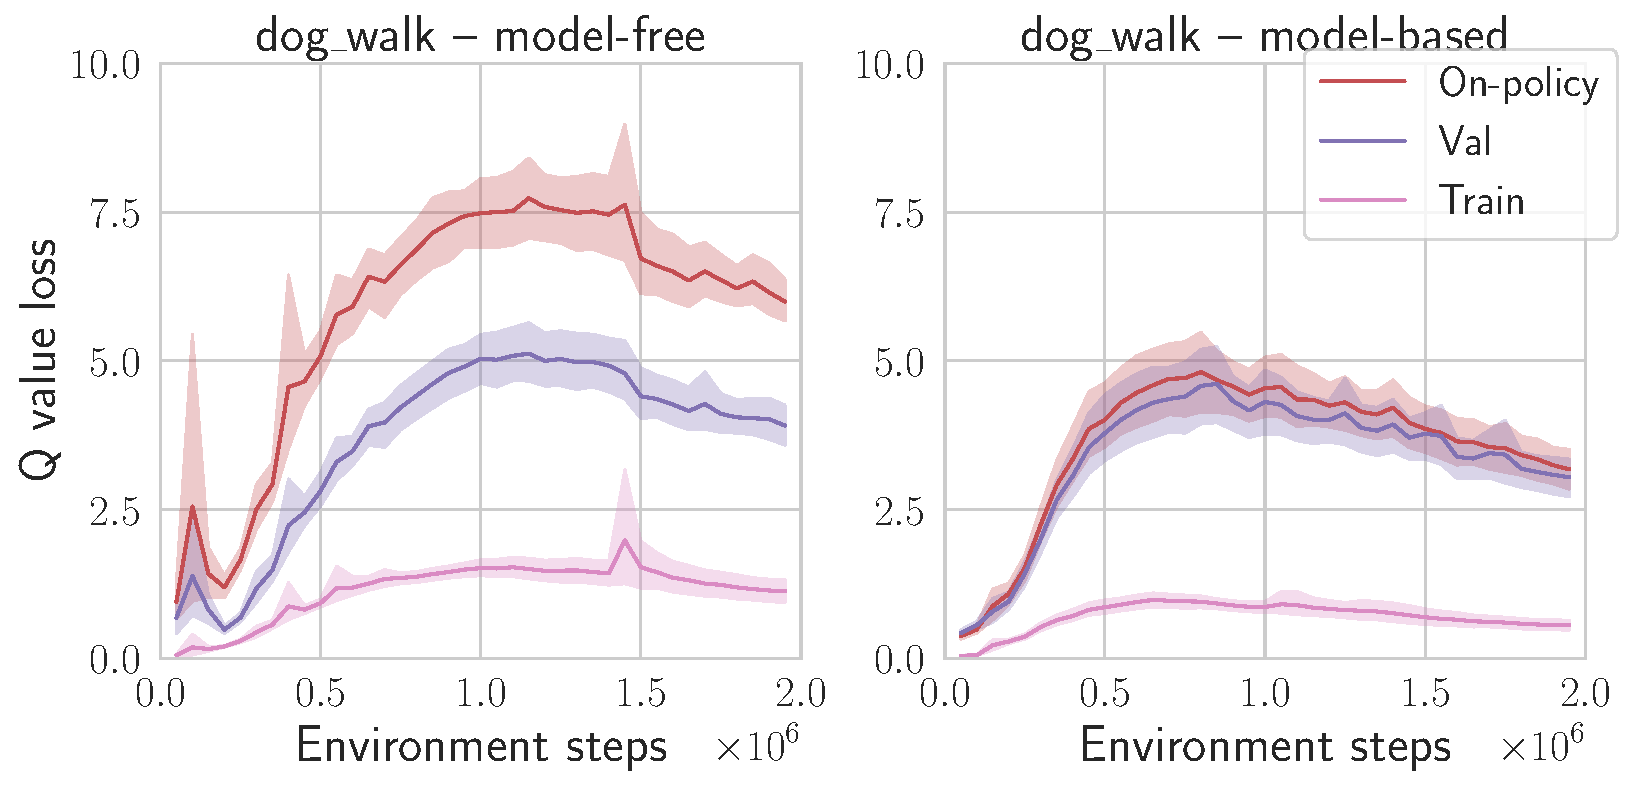
\includegraphics[width=0.5\textwidth]{figures/mad-td/critic_loss_dog_walk_model_based_separate.pdf}
    \caption{Average loss values with and without the model generated data (compare \autoref{fig:mad:q_eval}) at UTD 1.}
    \label{fig:mad:exp_repeat}    
\end{wrapfigure}
\textbf{Performance with and without model data at varying UTD ratios:}~~~
\begin{figure}[b]
    \centering
    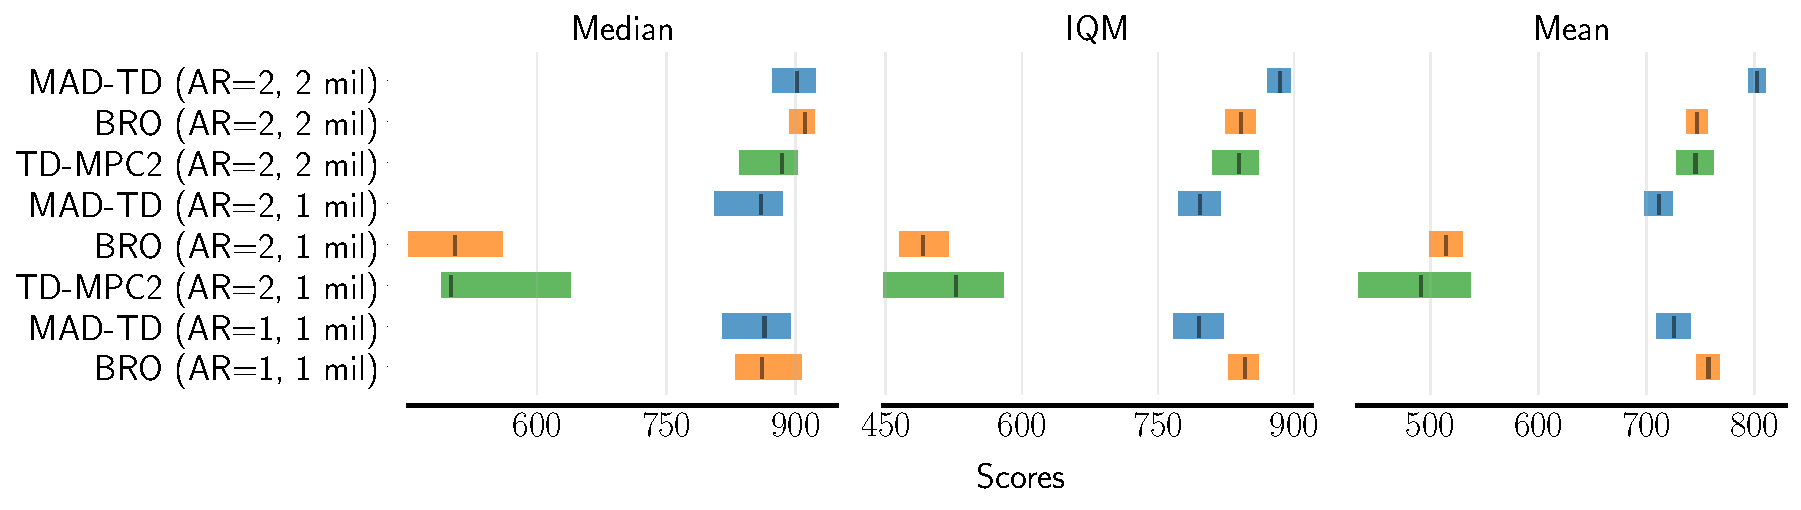
\includegraphics[width=1.\linewidth]{figures/mad-td/hard_rliable_comp.pdf}
    \caption{Performance comparison on the hard tasks for \sbcblue{MAD-TD}, \sbcorange{BRO}, and \sbcgreen{TD-MPC}, with varying number of steps and action repeat settings. MAD-TD is on par with all baselines, has higher mean and IQM when trained for 2 million time steps and action repeat 2, and strongly outperforms TD-MPC2 and BRO at 1 million time steps with action repeat 2.}
    \label{fig:mad:comp_baseline}
\end{figure}
In \autoref{fig:mad:main_dog} we present the impact of using model-based data across different UTD ratios.
Humanoid results are found in \autoref{app:results_hum}.
As is directly evident, across the dog tasks, we observe stagnating or deteriorating performance when increasing the update ratio, consistent with reports in prior work.
However, when using a small fixed amount of model generated data, this trend is reversed across all tested environments, with performance improving or at least remaining consistent.
We find that with model-based data, training is stable across a range of UTDs, even beyond those tested in recent high UTD work \parencite{nauman2024bigger}.
We also note that we observe only limited benefits from increasing the UTD ratio when properly mitigating \emph{misgeneralization}, except for the highly challenging dog run task, all other tasks perform on par with each other.

\textbf{Comparison with baselines:}~~~
As our method combines model-free and model-based updates, we compare our method against both TD-MPC2 \parencite{hansen2024tdmpc}, a strong model-based baseline, and BroNet \parencite{nauman2024bigger}, a recent algorithm proposed for high UTD learning.
Since \textcite{nauman2024bigger} and \textcite{hansen2024tdmpc} trained with differing numbers of action repeats, and we found that the performance does not cleanly translate between these regimes, we present our method both with an action repeat value of 1 and 2.
Some hyperparameters are adapted to the AR=1 setting (compare \autoref{tab:hyperparams}).
The results are presented in aggregate in \autoref{fig:mad:comp_baseline}, with per environment curves show in \autoref{app:results_base}.
We find that our method performs on par or above previous methods, and strikingly it is able to achieve higher returns faster than both TD-MPC2 and BRO.

\begin{figure}[t]
    \centering
    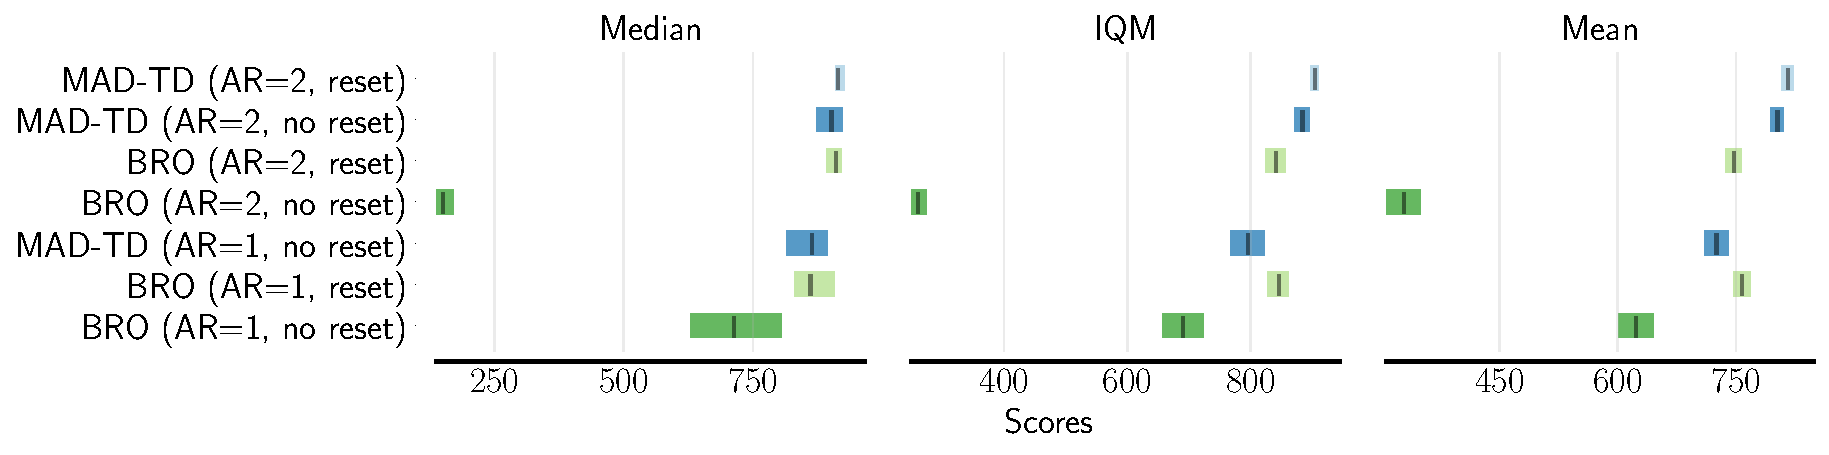
\includegraphics[width=1.\linewidth]{figures/mad-td/reset_rliable_comp.pdf}
    \caption{Resetting evaluation of \sbcblue{MAD-TD} and \sbcgreen{BRO}. Lighter color denotes performance with reset, and darker without. While MAD-TD's performance only increases slightly when adding resetting, BRO is unable to achieve strong performance in and setting without resetting.}
    \label{fig:mad:comp_reset}
\end{figure}

\subsection{Performance and stability impact of resetting}


\textbf{Resetting comparison:}~~~To investigate whether our technique benefits from more stable training, we set up a comparison in which we test the effects of resetting on our method. \autoref{fig:mad:comp_reset} presents aggregate results comparing our approach and BRO, both with and without resetting. 
Across all tasks we find that resetting barely improves MAD-TDs performance with the tested hyperparameters and update steps.
Benefits can only be observed on some seeds and can most likely be attributed to restarting the exploration process \parencite{hussing2024dissecting}.
However, the BRO algorithm is not able to achieve reliable performance without resets.
Overall, these results highlight that our model substantially improves the problems related to incorrect generalization of the value function, and that these are likely a major cause of the failure of high UTD learning in the DMC tasks.
Conjectured problems like the primacy bias effect~\parencite{nikishin2022primacy} need to be carefully investigated as we do not find evidence that a primacy bias impacts MAD-TD's performance in the DMC environments. 
Our work of course does not preclude the existence of phenomena such as loss of stability in different environments, architectures, or training setups. More discussion on this can be found in \autoref{app:related_work}.
\begin{wrapfigure}{r}{0.26\textwidth}
    \centering
    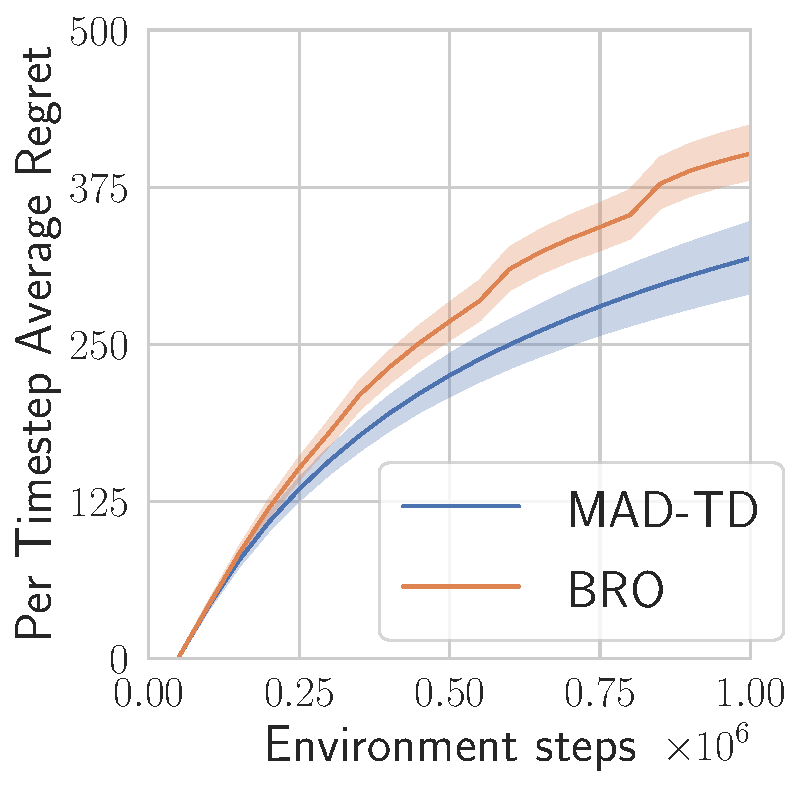
\includegraphics[width=0.26\textwidth]{figures/mad-td/average_regret_all_envs.pdf}
    \caption{Average regret ($\downarrow$), mean over the hard suite. Lower regret corresponds to faster, more stable training. \sbcblue{MAD-TD} outperforms \sbcorange{BRO}.}
    \label{fig:mad:regret}    
\end{wrapfigure}
%Our work of course does not preclude the existence of phenomena such as loss of stability in different environments, architectures, or training setups. More discussion on this can be found in \autoref{app:related_work}.

\textbf{Continued training:}~~~To highlight the pitfalls of resets, we employ a common RL theory metric the per timestep average regret
\begin{equation*}
    \overline{\text{Reg}}(T) = \frac{1}{T} \sum\nolimits_{t=0}^{T-1} \left(\mathcal{R}^* - \mathcal{R}_t\right) \enspace,
\end{equation*}
where $\mathcal{R}_t$ denotes the cumulative return in episode $t$ and $\mathcal{R}^*$ the optimal return. We use the maximum return any of the algorithms achieved $\hat{\mathcal{R}}^*$  as a lower bound on the optimal return $\mathcal{R}^*$. Regret quantifies how much better the algorithm could have performed throughout training. In other words, in situations where continued learning is crucial, such as many safety critical applications, regret might be a better measure of performance. It captures not only how good the final policy is, but also how well the algorithm adapts over time, and minimizes mistakes. We present a comparison of MAD-TD and the resetting-based BRO in~\autoref{fig:mad:regret} using an action repeat of $1$. The results show, even though both algorithms are close in their final return, their training behavior differs vastly. MAD-TD has lower regret showcasing its strength in continued deployment.

\subsection{Further experiments and ablations}
\label{sec:mad:adv_robustness}
\begin{figure}[t]
    \centering
    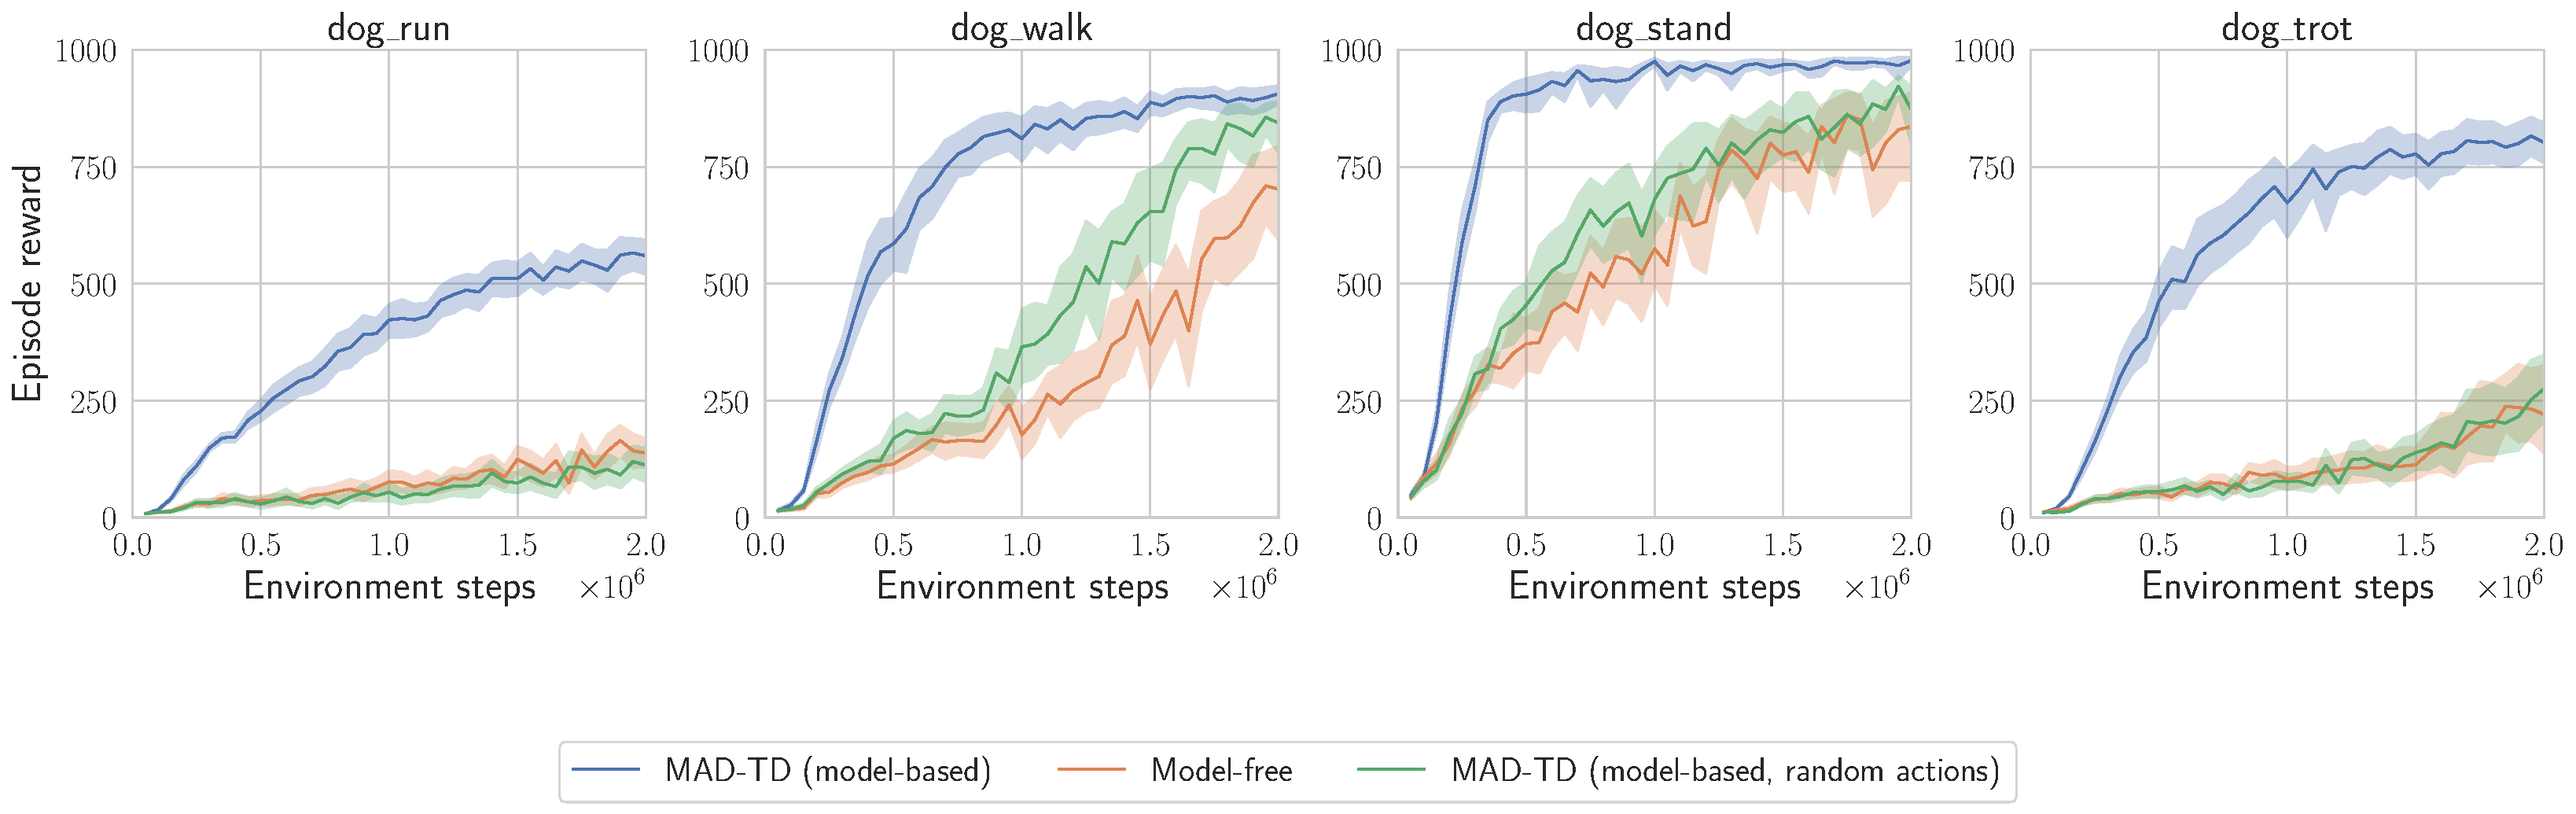
\includegraphics[width=1.\linewidth]{figures/mad-td/dog_random_actions.pdf}
    \caption{Return curves for the dog tasks when using \sbcblue{on-policy},  \sbcgreen{random} and  \sbcorange{no model-generated} data. When generating model-based data with random actions, performance of MAD-TD drops close to the model-free baseline, highlighting the importance of \emph{on-policy} actions.}
    \label{fig:mad:random_action}
\end{figure}

To further test our approach, we present two additional experiments on the \emph{hard suite}: changing the action selection for the model data generation, and reducing the model performance.
In addition, we investigate the impact of using model based data on the smoothness of the learned value function.

\textbf{Off-policy action selection in the model:}~~~To verify that the  improvement in performance is due to the off-policy correction provided by the model, we repeat the \emph{hard suite} experiments with a UTD of $8$ and $5\%$ model data, but we chose actions randomly from a uniform distribution across the action space.
The results are presented in \autoref{fig:mad:random_action}.
They highlight that random state-action pairs do not provide the necessary correction and the performance deteriorates to that of the model-free baseline.

\paragraph{Smaller model networks:}To study the effect of the modelling capacity on our method, we ablate the size of the latent model by reducing the network size across the hard suite.
\begin{figure}[b]
    \centering
    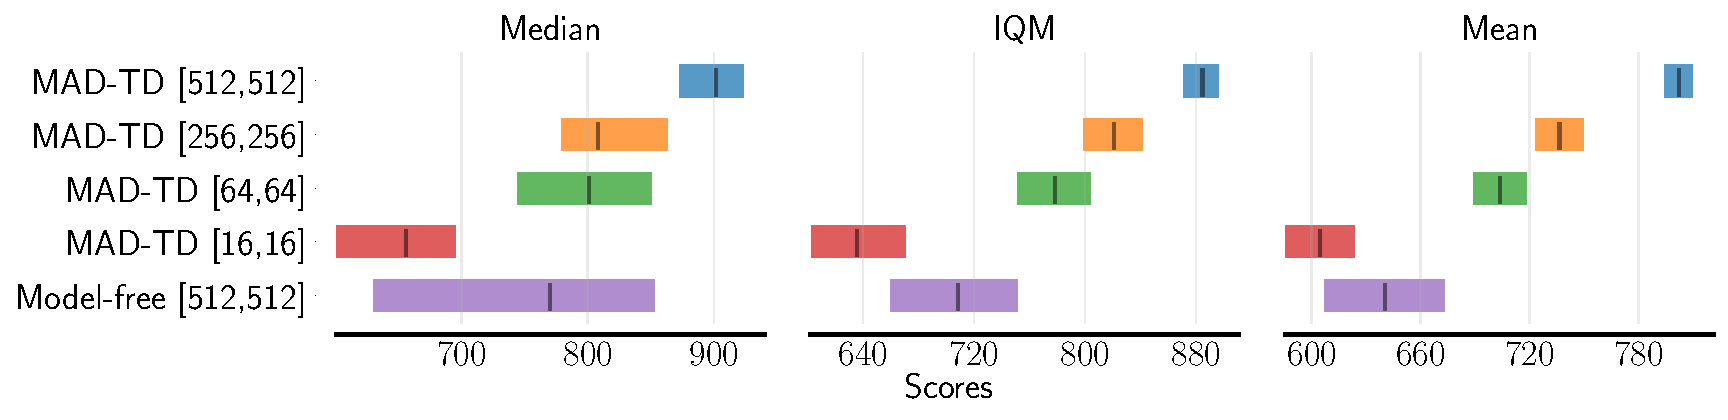
\includegraphics[width=1.0\linewidth]{figures/mad-td/model_ablation_rliable.pdf}
    \caption{Performance evaluation when reducing the model size of the latent model in MAD-TD. The performance predictably drops with decreasing hidden layer size, however only strongly decreasing the model size below 64 reduces the performance below that of the model-free ablation.}
    \label{fig:mad:model_ablation}
\end{figure}
The results are presented in \autoref{fig:mad:model_ablation}.
We see that reducing the network size has an immediate and monotonic impact on the performance of our approach, suggesting that the model learning accuracy and prediction capacity is indeed vital for our approach to function well.
However, even with small models of 64 hidden units, we still see some benefits from training with the model predicted data.

\begin{figure}[t]
    \centering
    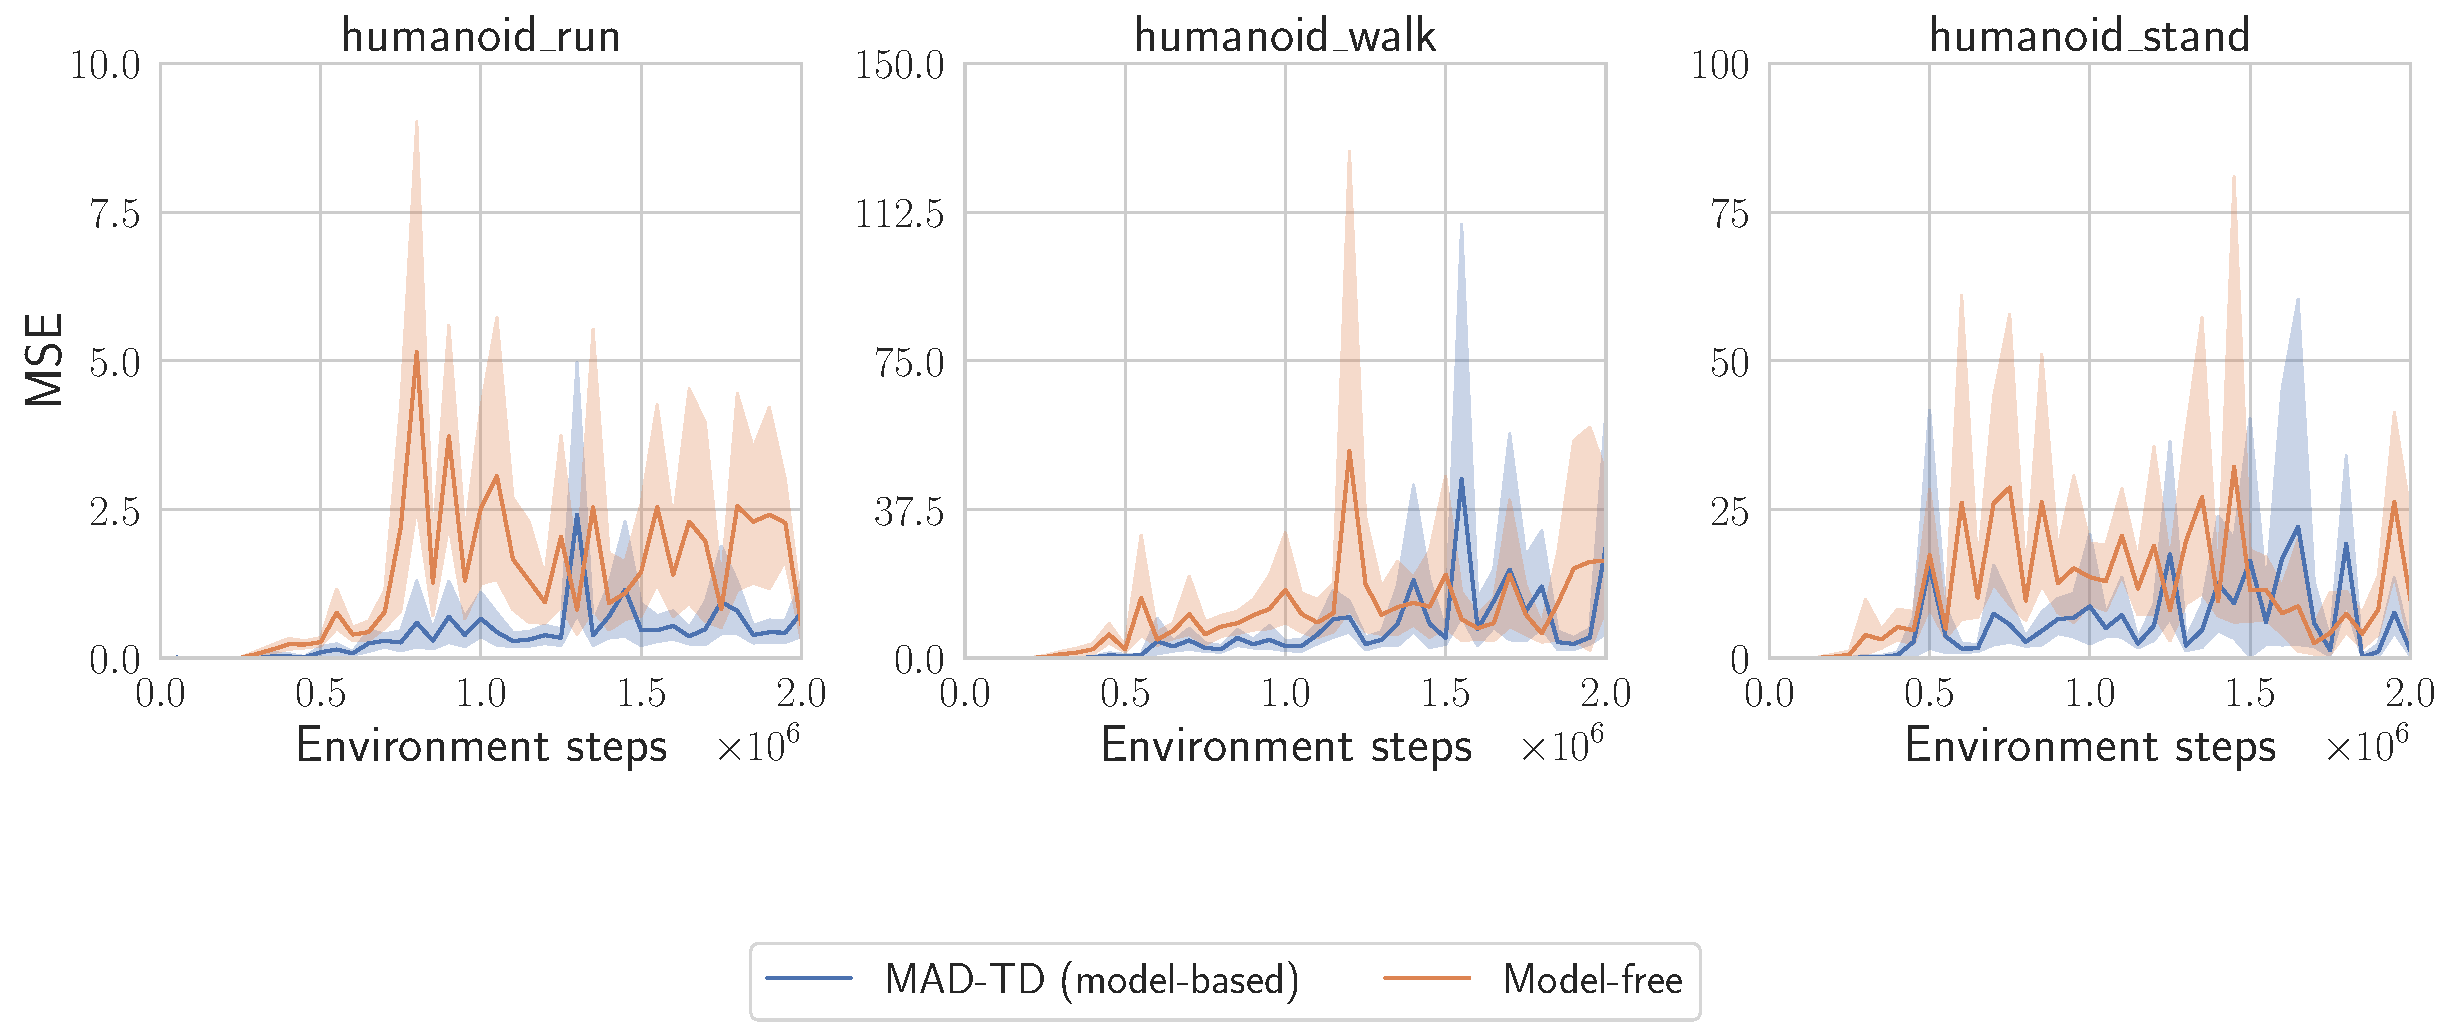
\includegraphics[width=0.75\linewidth]{figures/mad-td/adv_examples.pdf}
    \caption{Magnitude of the difference between $Q(x,\pi(x))$ and $Q(x,\tilde{a})$, where $\tilde{a}$ is an adversarial perturbation of $\pi(x)$. Across the training why see higher perturbation magnitude for the runs without model correction data.}
    \label{fig:mad:adv}
\end{figure}

\textbf{Perturbation robustness of the model-corrected value function:}~~~To motivate our method, we conjectured that one of the problems of training in actor-critic learning is that the actor is conducting a quasi adversarial search for overestimated values on the learned critic.\footnote{\emph{Quasi} because the actor is not constrained to find an action close to the replay buffer sample.}
To substantiate this claim and provide additional insight into the benefits of our approach, we used the iterated projected gradient method \cite{madry2018towards} to estimate the smoothness of the learned value functions across training on the humanoid environments at a UTD of 1 with and without model data.

Results are presented in \autoref{fig:mad:adv}.
Across the humanoid tasks we find that not using any model data leads to value functions with higher oscillations, either across the whole training run in \textsf{\small humanoid\_run}, or in the middle of training like in \textsf{\small stand} and \textsf{\small walk}.

\section{Conclusion}

Our experiments allow us to conclude that wrong generalization of the value functions to unseen, on-policy actions is indeed a major challenge that prevents stable off-policy RL, both in theory and in practice.
Model-Augmented Data for TD learning~(MAD-TD) is able to leverage the learning abilities of latent self-prediction models to provide small, yet crucial amounts of on-policy transitions which help stabilize learning across the hardest DeepMind Control suite tasks.
With a relatively simple model architecture and learning algorithm, this method proves to be on par with, or even outperform other strong approaches, and does not rely on mechanisms such as value function ensembles or resetting which were previously conjectured to be necessary for stable learning in high UTD regimes.

Our work opens up exciting avenues for future work.
The issue of poor generalization in off-policy learning can likely be tackled with other approaches such as diffusion models \parencite{lu2024synthetic} or better pretrained foundation models, and our presented experiments provide an important baseline for such work.
Furthermore, while we have purposefully kept our approach as simple as possible to validate our hypothesis, many ideas from the model-based RL community such as uncertainty quantification \parencite{pets,talvitie2024bounding}, multi-step corrections \parencite{buckman2018sample,hafner2020dream}, or policy gradient estimation \parencite{amos2021model} can be combined with our approach.
Our insight that surprisingly little data is necessary to achieve strong correction can likely be leveraged in these other approaches as well to trade-off model errors and value function errors more carefully.
Finally, while we chose the data to roll out in our models at random, our insights can likely be combined with ideas from the area of DYNA search control \parencite{pan2019hill,pan2020frequency} to select data points on which the correction has the most impact.
